\chapter{Advanced transverse coupling measurement} 
 \label{sec_coupling}

\begin{chapterinfo}
    The compensation of the driven motion is necessary for a reliable coupling measurement.
    This chapter introduces methods to compensate for driven beam motion in the calculation of
    coupling resonance driving terms. The methods currently applied in the LHC are revised and
    recent findings are presented.
\end{chapterinfo}

\section{Driven coupled motion}
In the past, two methods were used for coupling measurements in
the LHC, the first one uses only the difference in tunes to rescale the coupling terms. This is
a naive approach because it disregards the driven betatron phase but often this approximation is
good enough to get a first estimate of the coupling in the machine. We refer to this method as the
\emph{model method}.

The second method \cite{Miyamoto2010} applies the findings of a detailled study of the driven particle motion
which provides a compensation formula for all optics parameters that enter into the coupling terms. This method will
be called \emph{formula method} in the following.

Recent findings \cite{Carlier2020} show that the AC-dipole locally effects RDTs and introduces
a jump at its location. The detailled considerations of the formula method lack such an effect.
In view of the suggestions of \cite{Carlier2020} this work presents calculations of the terms
$f_{1001}$ and $f_{1010}$, building upon the techniques introduced in \ref{sec_driven_coords}.
A comparison between model method, formula method and the newly calculated coupling terms are shown.


\subsection{AC-dipole as skew quadrupole}

To start the section about the beam motion that is driven \emph{and} coupled, we state a curious
analogy between AC-dipole and skew quadrupoles.

Throughout this chapter we use the following convention:
%
\begin{align}
    f_+ &\equiv f_{0101} \text{ and}\notag \\
    f_- &\equiv f_{0110} 
    \fstop
\end{align}
%
The RDTs in \eqref{eq_f0101_f0110} can be reformulated:
%
\begin{equation}
    f_\pm = 
    \frac{
        \sum\limits_w J_{1,w} \sqrt{\beta_{x,w}\beta_{y,w}}
        \e{
            i\left[\varphi_{wj,x} \pm \varphi_{wj,y}\right]
            -i\pi\left[Q_x\pm Q_y\right]
        }
    }{
        8i\sin[\pi(Q_x\pm Q_y)]
    }
    \fstop
\end{equation}
%
The coupled motion for a single coupling source now reads
%
\begin{align}
    h_x(s_j,N) =& \zxp(s_j,N) \notag \\
    &+2i\frac{
         J_{1,w} \sqrt{\beta_{x,w}\beta_{y,w}}
    }{
        8i\sin[\pi(Q_x + Q_y)]
    }
    \zyp(s_j,N)
        \e{
            i\left[\Delta\phi_x^+ + 2\pi Q_x \Theta(s_j,s_w) + 2\pi Q_y \Theta(s_j,s_w)\right]
            -i\pi\left[Q_x + Q_y\right]
        }
        \notag \\
    &+2i\frac{
         J_{1,w} \sqrt{\beta_{x,w}\beta_{y,w}}
    }{
        8i\sin[\pi(Q_x - Q_y)]
    }
    \zym(s_j,N)
        \e{
            i\left[\Delta\phi_x^- + 2\pi Q_x \Theta(s_j,s_w) - 2\pi Q_y \Theta(s_j,s_w)\right]
            -i\pi\left[Q_x - Q_y\right]
        }
        \komma
\end{align}
%
with 
%
\begin{equation}
    \Delta\phi_x^\pm = \varphi_x(s_j) - \varphi_x(s_w) \pm \left(\varphi_y(s_j) - \varphi_y(s_w)\right)
    \fstop
\end{equation}
%
The $\Theta(s_j,s_w)$ terms come from the wrapping around of the phase advance. Noting that 
$\zyp(s_j,N) = \sqrt{2I_y}\e{2\pi i N Q_y + \varphi(s_j)}$
one can bring this in a form similar to \eqref{eq_forced_motion}
%
\begin{align}
    h_x(s_j,N) =& \zxp(s_j,N) \notag \\
    &+\frac{
         J_{1,w} \sqrt{\beta_{x,w}\beta_{y,w}}
    }{
        4\sin[\pi(Q_x + Q_y)]
    }
    \sqrt{2I_y}
    \e{
        2\pi i N Q_y + \varphi(s_j)
        +i\left[\Delta\phi_x^+ + 2\pi (Q_x+Q_y) \text{sgn}(s_w-s_j)\right]
    }
        \notag \\
    &+\frac{
        J_{1,w} \sqrt{\beta_{x,w}\beta_{y,w}}
    }{
        4\sin[\pi(Q_x - Q_y)]
    }
    \sqrt{2I_y}
    \e{
        -2\pi i N Q_y + \varphi(s_j)
        +i\left[\Delta\phi_x^- + 2\pi (Q_x-Q_y) \text{sgn}(s_w-s_j)\right]
    }
    \fstop
\end{align}
%
The following table summarises which quantities get replaced
\begin{center}
\begin{tabular}{ll}
    AC dipole & coupling \\
    \hline
    \hline
    $ A_\theta $        & $ J_{1,w} $ \\
    $ \varphi_x(s_d) $  & $ \varphi_y(s_j) - \varphi_y(s_w) \mp \varphi_x(s_w)$ \\
    $ \Qd{x} $          & $ Q_y $\\
    \hline
\end{tabular}
\end{center}
Thus, a single coupling source acts like an AC dipole with the tune of the other plane as driving frequency.
From another perspective, the AC dipole couples the beam's motion to its oscillation.

% --------------------------------------------------------------------------------------------------
% --- main part ------------------------------------------------------------------------------------
% --------------------------------------------------------------------------------------------------
\subsection{Derivation of the coupled driven motion}

The derivation of the coupled driven motion follows a similar path to the derivation of the 
coupled free motion but in the regime of driven motion, so the normal form approach has to be used.
Figure~\ref{fig_sketch_drv_ac} illustrates the procedure. The coordinates are propagated in normal form
space and transformed to physical space at $s_d-\epsilon$, directly in front of the AC-dipole. Then
an AC-dipole kick $\Delta h_x(N)$ is performed and the physical coordinate is transformed back to
normal form space where it is rotated around the ring. This process is repeated for each turn.

\begin{figure}
  \centering
  tikzpicture
      \caption{Kick performed in CS-coordinates, transformed to NF-coordinates}
  \label{fig_sketch_drv_ac}
\end{figure}

In the first turn, before the beam experiences the AC-dipole kick, the coordinates are those from
\eqref{eq_coupled_h_from_z}:
%
\begin{align}
  h_x^+(s_d-\epsilon, 0) &=  \e{\liemap{F}} \zeta_x^+(s_d-\epsilon, 0)\notag \\
  &=  \zeta^+(s_d-\epsilon,0)
    + 2i\conj{f_{1001}}\zeta_y^+(s_d-\epsilon, 0)
    + 2i\conj{f_{1010}}\zeta_y^-(s_d-\epsilon,0)
\end{align}
%
Then the particle is kicked in $p$ direction:
%
\begin{align}
  h_x^\pm(s_d+\epsilon, 0) =  h_x^\pm(s_d - \epsilon,0) + \Delta h_x^\pm(0)\notag \\
  h_y^\pm(s_d+\epsilon, 0) =  h_y^\pm(s_d - \epsilon,0) + \Delta h_y^\pm(0)
\end{align}
%
where the superscript $\pm$ of $\Delta h_z^\pm(N)$ denotes which of $h_z^+$ or $h_z^-$ is experiencing
the kick. The following holds:
%
\begin{equation}
    \Delta h_z^- = \conj{\left(\Delta h_z^+\right)} = -\Delta h_z^+
    \fstop
\end{equation}
%
For the transformation back to normal form space the inverse of \eqref{eq_h_from_z} has to be applied:
%
\begin{equation}
  \zeta = \e{\liemap{-F}} h = h + [-F,h] + O(h^3)
  \label{eq_coupled_h_after_kick}
\end{equation}
%
with
%
\begin{equation}
  F = \sum f_{jklm}\left( h_x^+ \right)^j \left( h_x^- \right)^k \left( h_y^+ \right)^l \left( h_y^- \right)^m
\end{equation}
%
when applied to $h_z^\pm$.
The normal form of the kicked particle motion now reads
%
\begin{align}
    \zeta_x^+(s_d+\epsilon, 0)
        &= h_x^+(s_d+\epsilon)
            - 2i\conj{f_{1001}}(s_d) \hyp(s_d+\epsilon, 0)
            - 2i\conj{f_{1010}}(s_d) \hym(s_d+\epsilon, 0)
    \notag\\
        &= \tilde{h}_x^+(s_d+\epsilon,0) + \Delta h_x(0)
            \notag \\ &\quad - 2i\conj{f_{1001}}(s_d) \left(\tilde{h}_y^+(s_d+\epsilon, 0) + \Delta h_y^+(0)\right)
            \notag \\ &\quad - 2i\conj{f_{1010}}(s_d) \left(\tilde{h}_y^-(s_d+\epsilon, 0) + \Delta h_y^-(0)\right)
    \notag \\
        &= \tilde{\zeta}_x^+(s_d+\epsilon, 0) + \Delta h_x(0)
            - 2i\conj{f_{1001}}(s_d) \Delta h_y^+(0)
            - 2i\conj{f_{1010}}(s_d) \Delta h_y^-(0)
\end{align}
%
where the tilde denotes undriven coordinates.
Propagation to the next turn is just a simple application of the transformation $R_x$, turning the
coordinate $\tilde{\zeta}_z^+(s,0)$ into $\tilde{\zeta}_z^+(s,1)$. The operator in front of $\Delta h_z$
is written out explicitely for now to avoid confusion. Its effect will be calculated later.
At turn 1, just in front of the AC-dipole, the particle's coordinate reads
%
\begin{align}
    \zxp(s_d-\epsilon, 1) &= R_x\zxp(s_d+\epsilon, 0) \notag \\
        &= \tilde{\zeta}_x^+(s_d-\epsilon, 1) + R_x\Delta h_x(0)
            - 2i\conj{f_{1001}}(s_d) R_x\Delta h_y^+(0)
            - 2i\conj{f_{1010}}(s_d) R_x\Delta h_y^-(0)
            \fstop
\end{align}
%
Before applying the AC-dipole kick it is again transformed to CS space:
%
\begin{align}
    \hxp(s_d-\epsilon, 1) &=R_x\zxp(s_d+\epsilon, 0) \notag \\
        &=
        \tilde{\zeta}_x^+(s_d-\epsilon, 1) + R_x\Delta h_x(0)
            - 2i\conj{f_{1001}}(s_d) R_x\Delta h_y^+(0)
            - 2i\conj{f_{1010}}(s_d) R_x\Delta h_y^-(0)
        \notag \\ &\quad 
            + 2i\conj{f_{1001}}(s_d) \left(\tilde{\zeta}_y^+(s_d-\epsilon, 1) + R_x\Delta h_y^+(0) \right)
        \notag \\ &\quad 
            + 2i\conj{f_{1010}}(s_d) \left(\tilde{\zeta}_y^-(s_d-\epsilon, 1) + R_x\Delta h_y^-(0) \right)
        \notag \\ &\quad
            + O(f^2)
        \komma
    \label{eq_cpl_drv_n1}
\end{align}
%
where $O(f^2)$ denotes quadratic and cross terms of $f_{1001}$ and $f_{1010}$. 
A kick $\Delta h_x(1)$ is applied and this procedure can be continued to arbitrary order N.
To avoid lengthy expressions, the driven uncoupled coordinates $h_z^{d\pm}$ are defined as
%
\begin{align}
    h_z^{d\pm} = \tilde{h}_z^{\pm} 
    +\frac{A_\theta}{4\sin(\pi Q_z^-)} \Bigg\{&
    \e{\pm i\left[-2N\pi Q_z^d - \varphi_{s_ds} + \pi Q_z^-\text{sgn}(s-s_d)\right]}
    \notag\\
    &- \lambda_z\e{\pm i\left[2N\pi Q_z^d - \varphi_{s_ds} - \pi Q_z^+\text{sgn}(s-s_d)\right]}
    \Bigg\}
\end{align}
%
where the sum up to turn $N$ has already been carried out as in section~\ref{sec_driven_coords}.
Note that the transformation from CS space to normal form space is carried out directly after the 
kick, thus fixing $f_{1001}$ and $f_{1010}$ acting on $Delta h_y^\pm$ to this position, i.e. $s_d$.
When calculating the CS coordinates at arbitrary position $s$, on the other hand, the RDTs acting on
$\zeta_y^\pm$ are evaluated at the position $s$. Therefore the coordinate, at position $s<s_d$ reads
%
\begin{align}
    \hxp(s<s_d, N) &= h_x^{d+}(s,N)
        + 2i\conj{f_{1001}}(s) h_y^{d+} (s, N)
        + 2i\conj{f_{1010}}(s) h_y^{d-} (s, N) \notag \\
        & \quad - 2i\conj{f_{1001}}(s_d) \sum\limits_{T = 1}^N R_{s-s_d}R_x^{T}\Delta h_y^+(N-T) \notag \\
        & \quad - 2i\conj{f_{1010}}(s_d) \sum\limits_{T = 1}^N R_{s-s_d}R_x^{T}\Delta h_y^-(N-T)
        \komma
        \notag \\
\end{align}
%
and, after the AC-dipole,
%
\begin{align}
    \hxp(s>s_d, N) &= h_x^{d+}(s,N)
        + 2i\conj{f_{1001}} h_y^{d+} (s, N)
        + 2i\conj{f_{1010}} h_y^{d-} (s, N) \notag \\
        & \quad - 2i\conj{f_{1001}}(s_d) \sum\limits_{T = 0}^N R_{x,s-s_d}R_x^{T}\Delta h_y^+(N-T) \notag \\
        & \quad - 2i\conj{f_{1010}}(s_d) \sum\limits_{T = 0}^N R_{x,s-s_d}R_x^{T}\Delta h_y^-(N-T)
        \fstop
\end{align}
%
The rotation $R_{x,s-s_d}$ is caused by the transfer of $\zeta_z^\pm$ to the position $s$,
before transformation into Courant-Snyder space is performed. 
The term $\sum\limits_{T = 0}^N R_x^{T}\Delta h_y^+(N-T) $ can be simplified as in section~\ref{sec_driven_coords}:
%
\begin{align}
    \sum\limits_{T=0}^N R_x^T \Delta h_y^+(N-T)
        &=
        i\frac{A_\theta}{2} \left\{
            \sum\limits_{T=0}^N R_x \delta_{y+}^{N-T}
            +\sum\limits_{T=0}^N R_x \delta_{y-}^{N-T}
        \right\}
        \notag \\
        &=
        i\frac{A_\theta}{2} \left\{
            R_x^N\frac{1-(R_x^{-1}\delta_{y+})}{1-R^{-1}\delta_{y+}}
            +R_x^N\frac{1-(R_x^{-1}\delta_{y-})}{1-R^{-1}\delta_{y-}}
        \right\}
        \notag \\
        &=
        \frac{A_\theta}{4} \left\{
            \frac{1-\e{2\pi i N\left[ Q_x + Q_y^d \right]}}{\e{i\pi \left[Q_x+Q_y^d\right]}\sin\left[\pi (Q_x+Q_y^d)\right]}
            -\frac{1-\e{-2\pi i N\left[ Q_y^d - Q_x \right]}}{\e{i\pi \left[Q_y^d-Q_x\right] }\sin\left[\pi (Q_y^d-Q_x)\right]}
        \right\}
        .
\end{align}
%
For the term $\sum\limits_{T = 0}^N R_x^{T}\Delta h_y^-(N-T) $ a similar process is performed, noting that
the action of $R_x^N$ now is 
%
\begin{equation}
R^N\Delta h_y^- = \e{-2 i \pi N Q_x} \Delta h_y^-
\fstop
\end{equation}
%
Combining the above, the expression for the coupled driven motion becomes
%
\begin{align}
    h_x^+(s,N)&=
    h_x^{d+}(s,N) + 2if^{*}_{1001}  h_y^{d+}(s,N) + 2if^{*}_{1010} h_y^{d-} \notag \\
    &\quad
    -2if^*_{1001}(s_d) h_{y,x}^+(s,N)
    -2if^*_{1010}(s_d) h_{y,x}^-(s,N)
    \komma
\end{align}
with the definition
%
\begin{align}
    h_{y,x}^\pm(s,N) &= 
        \frac{A_\theta}{4} \Bigg\{
             \frac{\e{\pm i \left[-2N \pi Q_y^d + \pi( Q_y^d - Q_x )\text{sgn}(s-s_d) - \varphi_{s_ds}^{x}\right]}}
                {\sin\left[\pi (Q_y^d - Q_x)\right]}
                \notag \\  & \quad\quad\quad
            -\frac{\e{ \pm i \left[2N\pi Q_y^d - \pi( Q_y^d + Q_x )\text{sgn}(s-s_d) - \varphi_{s_ds}^{x}\right]}}
                {\sin\left[\pi (Q_y^d + Q_x)\right]}
        \Bigg\}
        \fstop
    %\notag \\
    %&=
    %\frac{A_\theta}{4\sin\left[\pi(Q_y^d +Q_x)\right]} 
    %\notag \\ &\quad \times
    %\left(
    %   \e{i \left[2N \pi Q_y^d + \pi( Q_y^d + Q_x )\text{sgn}(s-s_d) + \varphi_{s_ds}\right]}
    %   +\lambda_c\e{i \left[-2N\pi Q_y^d + \pi( Q_y^d - Q_x )\text{sgn}(s-s_d)+ \varphi_{s_ds}\right]}
    %\right)
\end{align}
%
%with the corresponding $\lambda$. This can be brought into a general from
%%
%\begin{align}
%    h_{y,x}(s,N)= ...
%\end{align}
%
In section~\ref{sec_coupling_measurement} a way to measure coupling in realistic conditions is introduced.
In order to get the new driven RDT, $f_{1001}^\text{drv}$, one can look at the result of a theoretical
measurement without calibration errors and with perfect knowledge of the complex signal.
Under these conditions one can get $f_{1001}$ from the free motion by (cf. \eqref{eq_hxpm_hypm})
%
\begin{equation}
    f_{1001}^* = \frac{H^+(0,1)}{2iV^+(0,1)}
    \label{eq_f1001_from_complex}
    \fstop
\end{equation}
%
In the driven case, on the other hand, the coordinates change $h_z^\pm \rightarrow h_z^{d\pm}$, which
causes also the generating terms to change $f_{jklm} \rightarrow f^d_{jklm}$ and, finally, the kick
cross-terms pollute the driven motion.
The easier term to calculate in \eqref{eq_f1001_from_complex} is $V^+(0,1)$
%
\begin{align}
    V^+(0,1) &= \four{h_y^+}(Q_y^d) = \four{h_y^{d+}}(Q_y^d)
    \notag \\
    &= \frac{A_\theta}{4\sin(\pi Q_y^-)}
        \e{i\left[-\varphi_{s_ds}^{y} + \pi Q_y\text{sgn}(s-s_d)\right]}
        \fstop
\end{align}
%
$H^+(0,1)$, however, includes many terms proportional to $\e{-i\pi N Q_y^d}$:
%
\begin{align}
   H^+(0,1) &=
    2i \conj{f_{1001}}      \four{h_y^{d+}}(Q_y^d)
   +2i \conj{f_{1010}}      \four{h_y^{d-}}(Q_y^d)
   \notag \\&\quad
   -2i \conj{f_{1001}}(s_d) \four{h_{y,x}^{+}}(Q_y^d)
   -2i \conj{f_{1010}}(s_d) \four{h_{y,x}^{-}}(Q_y^d)
\end{align}
%
For readability the fourier transforms are listed seperately:
%
\begin{align}
    \four{h_y^{d+}}(Q_y^d) &= \frac{A_\theta}{4\sin\pi Q_y^-}
        \e{i\left[-\varphi_{s_ds}^{y} + \pi Q_y^-\text{sgn}(s-s_d)\right]}
    \komma
    \notag \\
    \four{h_y^{d-}}(Q_y^d) &= \frac{\lambda_y A_\theta}{4\sin\pi Q_y^-}
        \e{i\left[\varphi_{s_ds}^{y} + \pi Q_y^+\text{sgn}(s-s_d)\right]}
    \komma
    \notag \\
    \four{h_{y,x}^{+}}(Q_y^d) &= \frac{A_\theta}{4\sin\left[\pi (Q_y^d - Q_x)\right]}
        \e{i\left[-\varphi_{s_ds}^{x} + \pi (Q_y^d - Q_x)\text{sgn}(s-s_d)\right]}
    \komma
    \notag \\
    \four{h_{y,x}^{-}}(Q_y^d) &= \frac{A_\theta}{4\sin\left[\pi (Q_y^d + Q_x)\right]}
        \e{i\left[\varphi_{s_ds}^{x} + \pi (Q_y^d + Q_x)\text{sgn}(s-s_d)\right]}
    \fstop
\end{align}
%
From this it is easy to calculate the driven coupling term 
%
\begin{align}
    f_{1001}^{\text{drv}*} &=
    f_{1001}^*
    + f_{1001}^*(s_d) \frac{\sin\pi Q_y^-}{\sin\left[\pi (Q_y^d-Q_x)\right]}
        \e{i\left[\varphi_{s_ds}^{x} -\varphi_{s_ds}^{y} + \pi(Q_y-Q_x)\text{sgn}(s-s_d)\right]}
        \notag \\
    &\quad
    + \lambda_y f_{1010}^*\e{2i\left[ \varphi_{s_ds}^{y} + \pi Q_y\right]}
    + f_{1010}^*(s_d) \frac{\sin\pi Q_y^-}{\sin\left[\pi (Q_y^d+Q_x)\right]}
        \e{i\left[\varphi_{s_ds}^{x} + \varphi_{s_ds}^{y} + \pi(Q_y+Q_x)\text{sgn}(s-s_d)\right]}
    \label{eq_drv_f1001_final}
\end{align}

% --------------------------------------------------------------------------------------------------
\subsection{Model and Formula methods}

For the sake of completeness, model and formula methods will be stated here. The detailled derivation
can be looked up in the respective publications \cite{Miyamoto2008}.

The compensation by model simply rescales the coupling terms $f_{1001}$ and $f_{1010}$ by their expected
denominators:
%
\begin{align}
    f_{1001} &= \frac{\sin(\Qd{y} - Q_x) \sin(\Qd{x} - Q_y)}{\sin(Q_x-Q_y)}f_{1001}^\text{drv}
    \notag \\
    f_{1010} &= \frac{\sin(\Qd{y} + Q_x) \sin(\Qd{x} + Q_y)}{\sin(Q_x+Q_y)}f_{1010}^\text{drv}
    \fstop
\end{align}
%
For the formula method, a complete expression for the driven RDTs can be derived:
%
\begin{align}
    f_{\pm,x} = \frac{1}{\sqrt{1-\lambda_x^2}}
        \frac{
            \sin\left[\pi(Q_x\mp Q_y)\right]
        }{
            \sin\left[\pi(\Qd{x}\mp Q_y)\right]
        }
        \Bigg\{&
        \e{i(\varphi_{s_ds}^{\text{d},x} - \varphi_{s_ds}^{x} )} f_{\mp}
        +\lambda_x \lambda_c \e{i(\varphi_{s_ds}^{\text{d},x} - \varphi_{s_ds}^{x} )}f_{\pm}^*
        \notag \\
        & +2i \sin(\pi(Q_x^-))\e{i(\varphi_{s_ds}^{\text{d},x} - \varphi_{s_ds}^{x} )}f_{\pm}(s;s,s_d)
        \notag \\
        & +2i \lambda_c^{\mp 1} \sin(\pi(Q_x^-))\e{i(\varphi_{s_ds}^{\text{d},x} + \varphi_{s_ds}^{x} )}f_{\mp}(s;s,s_d)
        \Bigg\}
        \komma
\end{align}
%
for the $f$~terms as measured from the signal in the horizontal plane, and
%
\begin{align}
    f_{\pm,y} = \frac{1}{\sqrt{1-\lambda_y^2}}
        \frac{
            \sin\left[\pi(Q_x\mp Q_y)\right]
        }{
            \sin\left[\pi(Q_x\mp \Qd{y})\right]
        }
        \Bigg\{&
        \e{i(\varphi_{s_ds}^{\text{d},x} - \varphi_{s_ds}^{x} )} f_{\mp}
        +\lambda_x \lambda_c \e{i(\varphi_{s_ds}^{\text{d},x} - \varphi_{s_ds}^{x} )}f_{\pm}^*
        \notag \\
        & +2i \sin(\pi(Q_x^-))\e{i(\varphi_{s_ds}^{\text{d},x} - \varphi_{s_ds}^{x} )}f_{\pm}(s;s,s_d)
        \notag \\
        & +2i \lambda_c^{\mp 1} \sin(\pi(Q_x^-))\e{i(\varphi_{s_ds}^{\text{d},x} + \varphi_{s_ds}^{x} )}f_{\mp}(s;s,s_d)
        \Bigg\}
        \komma
        \label{eq_drv_cpl_f_ryo}
\end{align}
%
from measurements in the vertical plane.
In order to simplify the expression, some extra definitions were introduced:
%
\begin{align}
    f_+ &= f_{1010}\komma\notag \\
    f_- &= f_{1001}\komma\notag \\
    \lambda_c &= \frac{\sin\left[\pi(Q_x-Q_y)\right]}{\sin\left[\pi(Q_x+Q_y)\right]}\komma
    \notag \\
    f_{\mp}(s_j;s_a,s_b) &= \frac{
        \sum\limits_{w\in I(s_a,s_b)} h_{w,\mp}\e{i[\varphi_{wj}^x \mp \varphi_{wj}^y]}
    }{
        1-\e{2\pi i [Q_x\mp Q_y]}
    }\komma
\end{align}
%
where the interval $I(s_a,s_b)$  contains all elements between $s_a$ and $s_b$,
%
\begin{equation}
    I(s_a,s_b) = \{w: s_a < s_w < s_b\},
\end{equation}
%
and for $h_{w,\mp}$ the same convention applies as for $f_\mp$.
Measurements can only be performed on the real signal and the complex signal needed for the calculation
of RDTs has to be reconstructed.  
This reconstruction mixes the RDTs $f_+$ and $f_-$, given by the following equation. Under the assumption
that adjacent BPMs are used for the reconstruction, the combined $f$~terms read
%
\begin{align}
   f_{\mp,x,y} = \frac{1}{\sqrt{1-\lambda_y^2}}
   \left\{
       \e{\pm i [\varphi^{\text{d},x}_{s_ds}] - \varphi^{x}_{s_ds}]}f_{\mp,x}
       - \lambda_y\e{\pm[\varphi^{\text{d},y}_{s_ds}] - \varphi^{y}_{s_ds}]}f_{\pm,x}
    \right\}
    \fstop
\end{align}
%
It is important to take into account this fact when finally reconstructing the driven $f$~terms from
the measured ones.

\subsection{Comparison of the methods for typical LHC machine configurations}

In this section the effect of the driven motion on the measured RDTs is studied. From \eqref{eq_driven_f1001_final}
one can see that the effect of the AC-dipole jump is proportional to the strength of the RDTs at the 
position of the AC-dipole. This means, given a weak initial coupling around the AC-dipole or a sufficient
correction of the local coupling, the effect is expected to be low and further coupling measurements
are not impacted by it. 

Given that the effect is only a minor one in the first place, repeated measurement and correction of
coupling will iteratively improve the precision of the coupling measurement.
%
\begin{figure}[h]
  \centering
  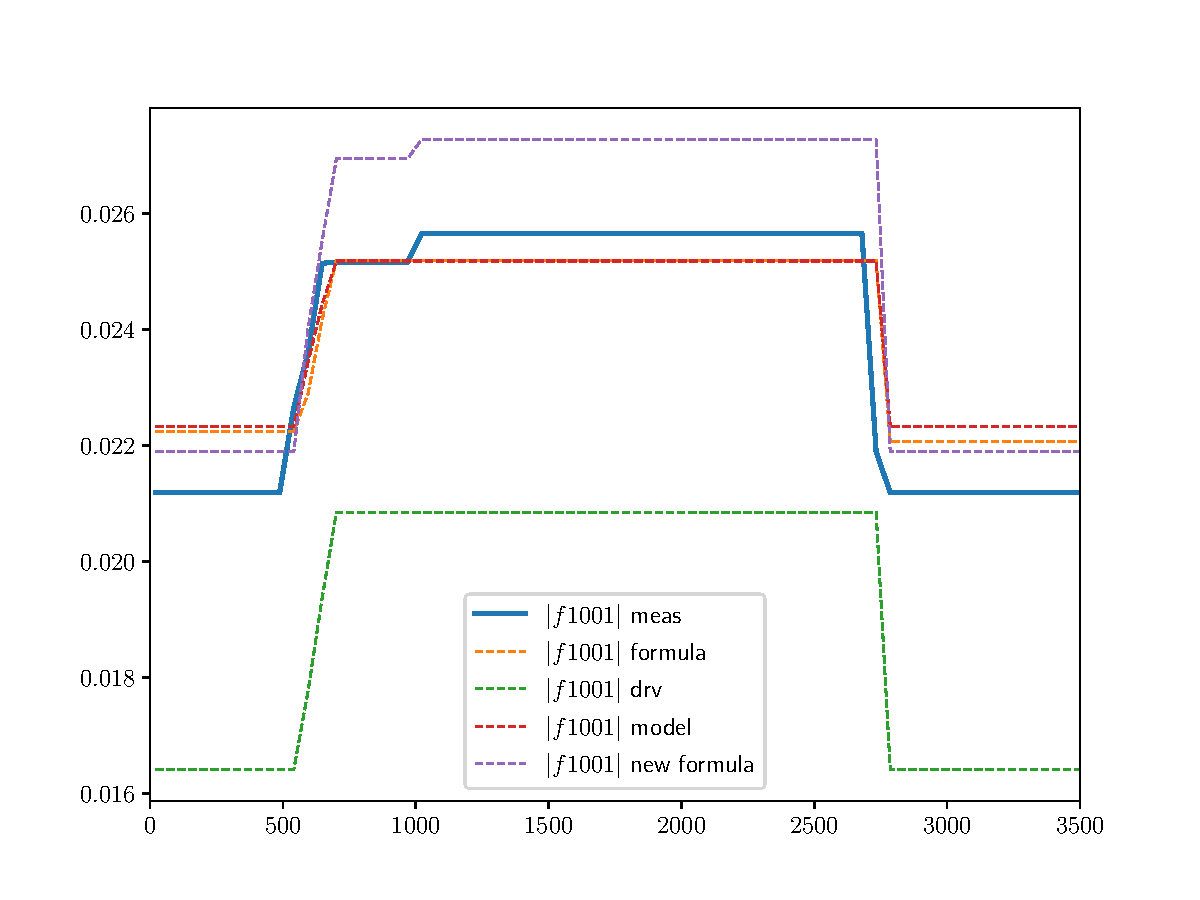
\includegraphics[width=.7\linewidth]{forced_rdts_abs}
  \caption{Comparison of the three methods with the AC-dipole surrounded by a coupling bump.
    The AC-dipole is creating a jump in the coupling term $f_{1001}$ at its location. Only the new
    formula is able to reproduce this jump.
  }
  \label{fig_comp_felix_ryo}
\end{figure}
%

Figure~\ref{fig_comp_felix_ryo} shows the comparison between the three methods.